\chapter{Analyse des résultats}
\par Dans cette partie nous allons analyser les résultats de chacun des algorithmes.
\section{Résultats}
\subsection{Régression logistique}
\subsection{SVM}
\par Les erreurs et les précisions d'entrainement et de test:
\begin{figure}[H]
    \centering
    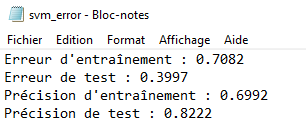
\includegraphics{svm.png}
    \caption{Figure SVM-error }
    \label{Figure fichier svm-error }
\end{figure}
\subsection{Réseaux de neuronnes}
\subsection{Bagging}
\subsection{AdaBoost} 
\par Pour "lr" entre 0.01 et 1, et pour "n-estimators" entre 1 et 101, les meilleurs valeurs pour les hyper-paramètres "lr" et "n-estimator" sont ceux affichés dans la figure 3.2
\begin{figure}[H]
    \centering
    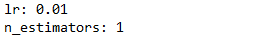
\includegraphics{adaboost_param.PNG}
    \caption{Figure adaboost-param }
    \label{Figure fichier adaboost-param }
\end{figure}
\par Les précisions d'entrainement et de test:
\begin{figure}[H]
    \centering
    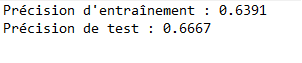
\includegraphics{adaboost.PNG}
    \caption{Figure adaboost-error }
    \label{Figure fichier adaboost-error }
\end{figure}
\section{Analyse}
